\documentclass[twocolumn,tighten,times]{aastex62}
%\documentclass[twocolumn,times]{aastex62}
%% The default is a single spaced, 10 point font, single spaced article.
%% There are 5 other style options available via an optional argument. They
%% can be envoked like this:
%%
%% \documentclass[twocolumn]{aastex62}
%% 
%% where the layout options are:
%%
%%  twocolumn   : two text columns, 10 point font, single spaced article.
%%                This is the most compact and represent the final published
%%                derived PDF copy of the accepted manuscript from the publisher
%%  manuscript  : one text column, 12 point font, double spaced article.
%%  preprint    : one text column, 12 point font, single spaced article.  
%%  preprint2   : two text columns, 12 point font, single spaced article.
%%  modern      : a stylish, single text column, 12 point font, article with
%% 		  wider left and right margins. This uses the Daniel
%% 		  Foreman-Mackey and David Hogg design.
%%  RNAAS       : Preferred style for Research Notes which are by design 
%%                lacking an abstract and brief. DO NOT use \begin{abstract}
%%                and \end{abstract} with this style.
%%
%% Note that you can submit to the AAS Journals in any of these 6 styles.
%%
%% There are other optional arguments one can envoke to allow other stylistic
%% actions. The available options are:
%%
%%  astrosymb    : Loads Astrosymb font and define \astrocommands. 
%%  tighten      : Makes baselineskip slightly smaller, only works with 
%%                 the twocolumn substyle.
%%  times        : uses times font instead of the default
%%  linenumbers  : turn on lineno package.
%%  trackchanges : required to see the revision mark up and print its output
%%  longauthor   : Do not use the more compressed footnote style (default) for 
%%                 the author/collaboration/affiliations. Instead print all
%%                 affiliation information after each name. Creates a much
%%                 long author list but may be desirable for short author papers
%%

\usepackage{xspace}  %  to preserve spaces following a control word

\newcommand{\vdag}{(v)^\dagger}
\newcommand\aastex{AAS\TeX}
\newcommand\latex{La\TeX}
\newcommand{\ia}{SN\,Ia\xspace}
\newcommand{\ias}{SNe\,Ia\xspace}
\newcommand\one{(C)ON\lowercase{e}M\lowercase{g}\xspace}

 
%% figures live in this folder 
\graphicspath{{./}{figures/}}



%\received{January 1, 2018}
%\revised{January 7, 2018}
%\accepted{\today}
\submitjournal{AAS Journals}
\shorttitle{Type Ia SNe from evolved helium stars}
\shortauthors{Antoniadis et al.}


\begin{document}

\title{TYPE Ia SUPERNOVAE FROM NON-ACCRETING HELIUM STARS}


\correspondingauthor{John Antoniadis}
\email{janton@mpifr.de}

\author[0000-0002-0786-7307]{John Antoniadis}

\affil{Max-Planck Institut f\"{u}r Radioastronomie, Auf dem H\"{u}gel 69, 53121, Bonn DE}
\affil{Argelander Institut f\"{u}r Astronomie,
Auf dem H\"{u}gel 71, 53121, Bonn DE}

\author{Savvas G. Chanlaridis}
\author{G\"{o}tz Gr\"{a}fener}
\author{Norbert Langer}
\affil{Argelander Institut f\"{u}r Astronomie, 
Auf dem H\"{u}gel 71, 53121, Bonn DE}

\begin{abstract}
  We consider the evolution of helium stars in the mass range $1.5 \leq M/{\rm M}_{\odot}\leq 3.5$
\end{abstract}


\keywords{stars: neutron --- stars: massive}


\section{Introduction} \label{sec:intro}
Type Ia supernovae (\ias{}) signal the  disruption of a star 
in a thermonuclear explosion. The prompt conversion of $\sim 1$\,M$_{\odot}$ of  
material into iron-group elements and the subsequent radioactive decay of $^{56}$Ni
ejecta, power a luminous transient that can shine across 
cosmological distances \citep[e.g.][]{Arnett:1982}. \ia light curves are 
also remarkably homogeneous, exhibiting a tight correlation between maximum luminosity and 
rate of decline \citep{Phillips:1993ng}. Considered together, these  salient properties make \ias 
unique cosmological distance indicators and valuable tools for probing the expansion history of the Universe \citep{Riess:1998cb,Perlmutter:1998np}. 

 Despite their central role in Astrophysics and Cosmology, 
 the origins and physics of \ia{} explosions are still debated. 
 \ia spectra, by definition, lack hydrogen and helium but have strong silicon and iron-group lines. 
 Considered together with their high luminosities which imply 
 ejecta masses (typically $\gtrsim 0.2$\,M$_{\odot}$), 
these spectral properties indicate  that \ia progenitors are 
 compact stellar cores that disrupt, rather than exploding 
 massive stars that eject their hydrogen-rich envelopes
 \citep[][and references therein]{Maoz:2013hna}. 
 Carbon/oxygen white dwarfs (CO WDs) approaching the Chandrasekhar limit 
 are promising progenitor systems, consistent with the observed 
 spectra and inferred energetics \citep{Arnett:1969,Wang:2012za,Maoz:2013hna}.
 
 In  typical \ia scenarios, matter accretion onto the WD is required to trigger the explosion, 
 either through stable mass transfer from a donor star,  or in a merger event.  
Thus far, none of these single- (SD) and double-degenerate (DD) models 
are without problems \citep{vanKerkwijk:2010he}. For instance SD models require significant 
fine-tuning of the mass accretion rate, and also predict 
interaction between the ejecta and the donor star, which has not yet 
been observed in early light curves. 
Similarly, super-Chandrasekhar DD models generally 
predict too few events, whereas lower-mass mergers may survive instead of exploding promptly. 

In this paper we discuss an alternative progenitor model
in which a low-mass He star evolves onto a near-Chandrasekhar mass 
oxygen-neon (ONe) or carbon-oxygen-neon (CONe) star, 
which then ignites oxygen before the onset of $e^{-}$-captures onto $^{20}$Ne.

 
%super-giant structure due to helium shell burning. We argue that 
%this likely leads to the complete removal of the He-rich envelope, 
%either via a super-Eddington wind or, mode likely, in an inevitable common-envelope episode. 
%As we shall see in Section\,\ref{sec:2}, 


\section{Formation of \one cores}\label{sec:2}
The formation of degenerate ONeMg cores has been investigated extensively, 
especially in the context of super-AGB evolution. 
\citep[for recent results see][]{Chen:2014,Denissenkov:2013qaa,Schwab:2015bma,Lecoanet:2016,Meyer:2017elq,Woosley:2019sdf}.
Generally, the evolution during and beyond core-helium burning in this regime is complicated and poorly understood. In this section, we briefly summarise some of the key aspects of (C)ONe core formation, which are most relevant to the discussion below. 

Most commonly, (C)ONe cores develop inside stars which are born with zero-age 
main-sequence (ZAMS) masses between $\sim 6$ and 9\,M$_{\odot}$ \citep{Farmer:2015afs}.

After core helium burning, the carbon-oxygen core cools efficiently via neutrino emission. 
As a result, the maximum temperature is attained off-centre, and eventually 
carbon ignites off-center and propagates initially toward the centre and then outwards 
in a series of degenerate flashes. The details of flame propagation 

\begin{figure*}
\begin{center}
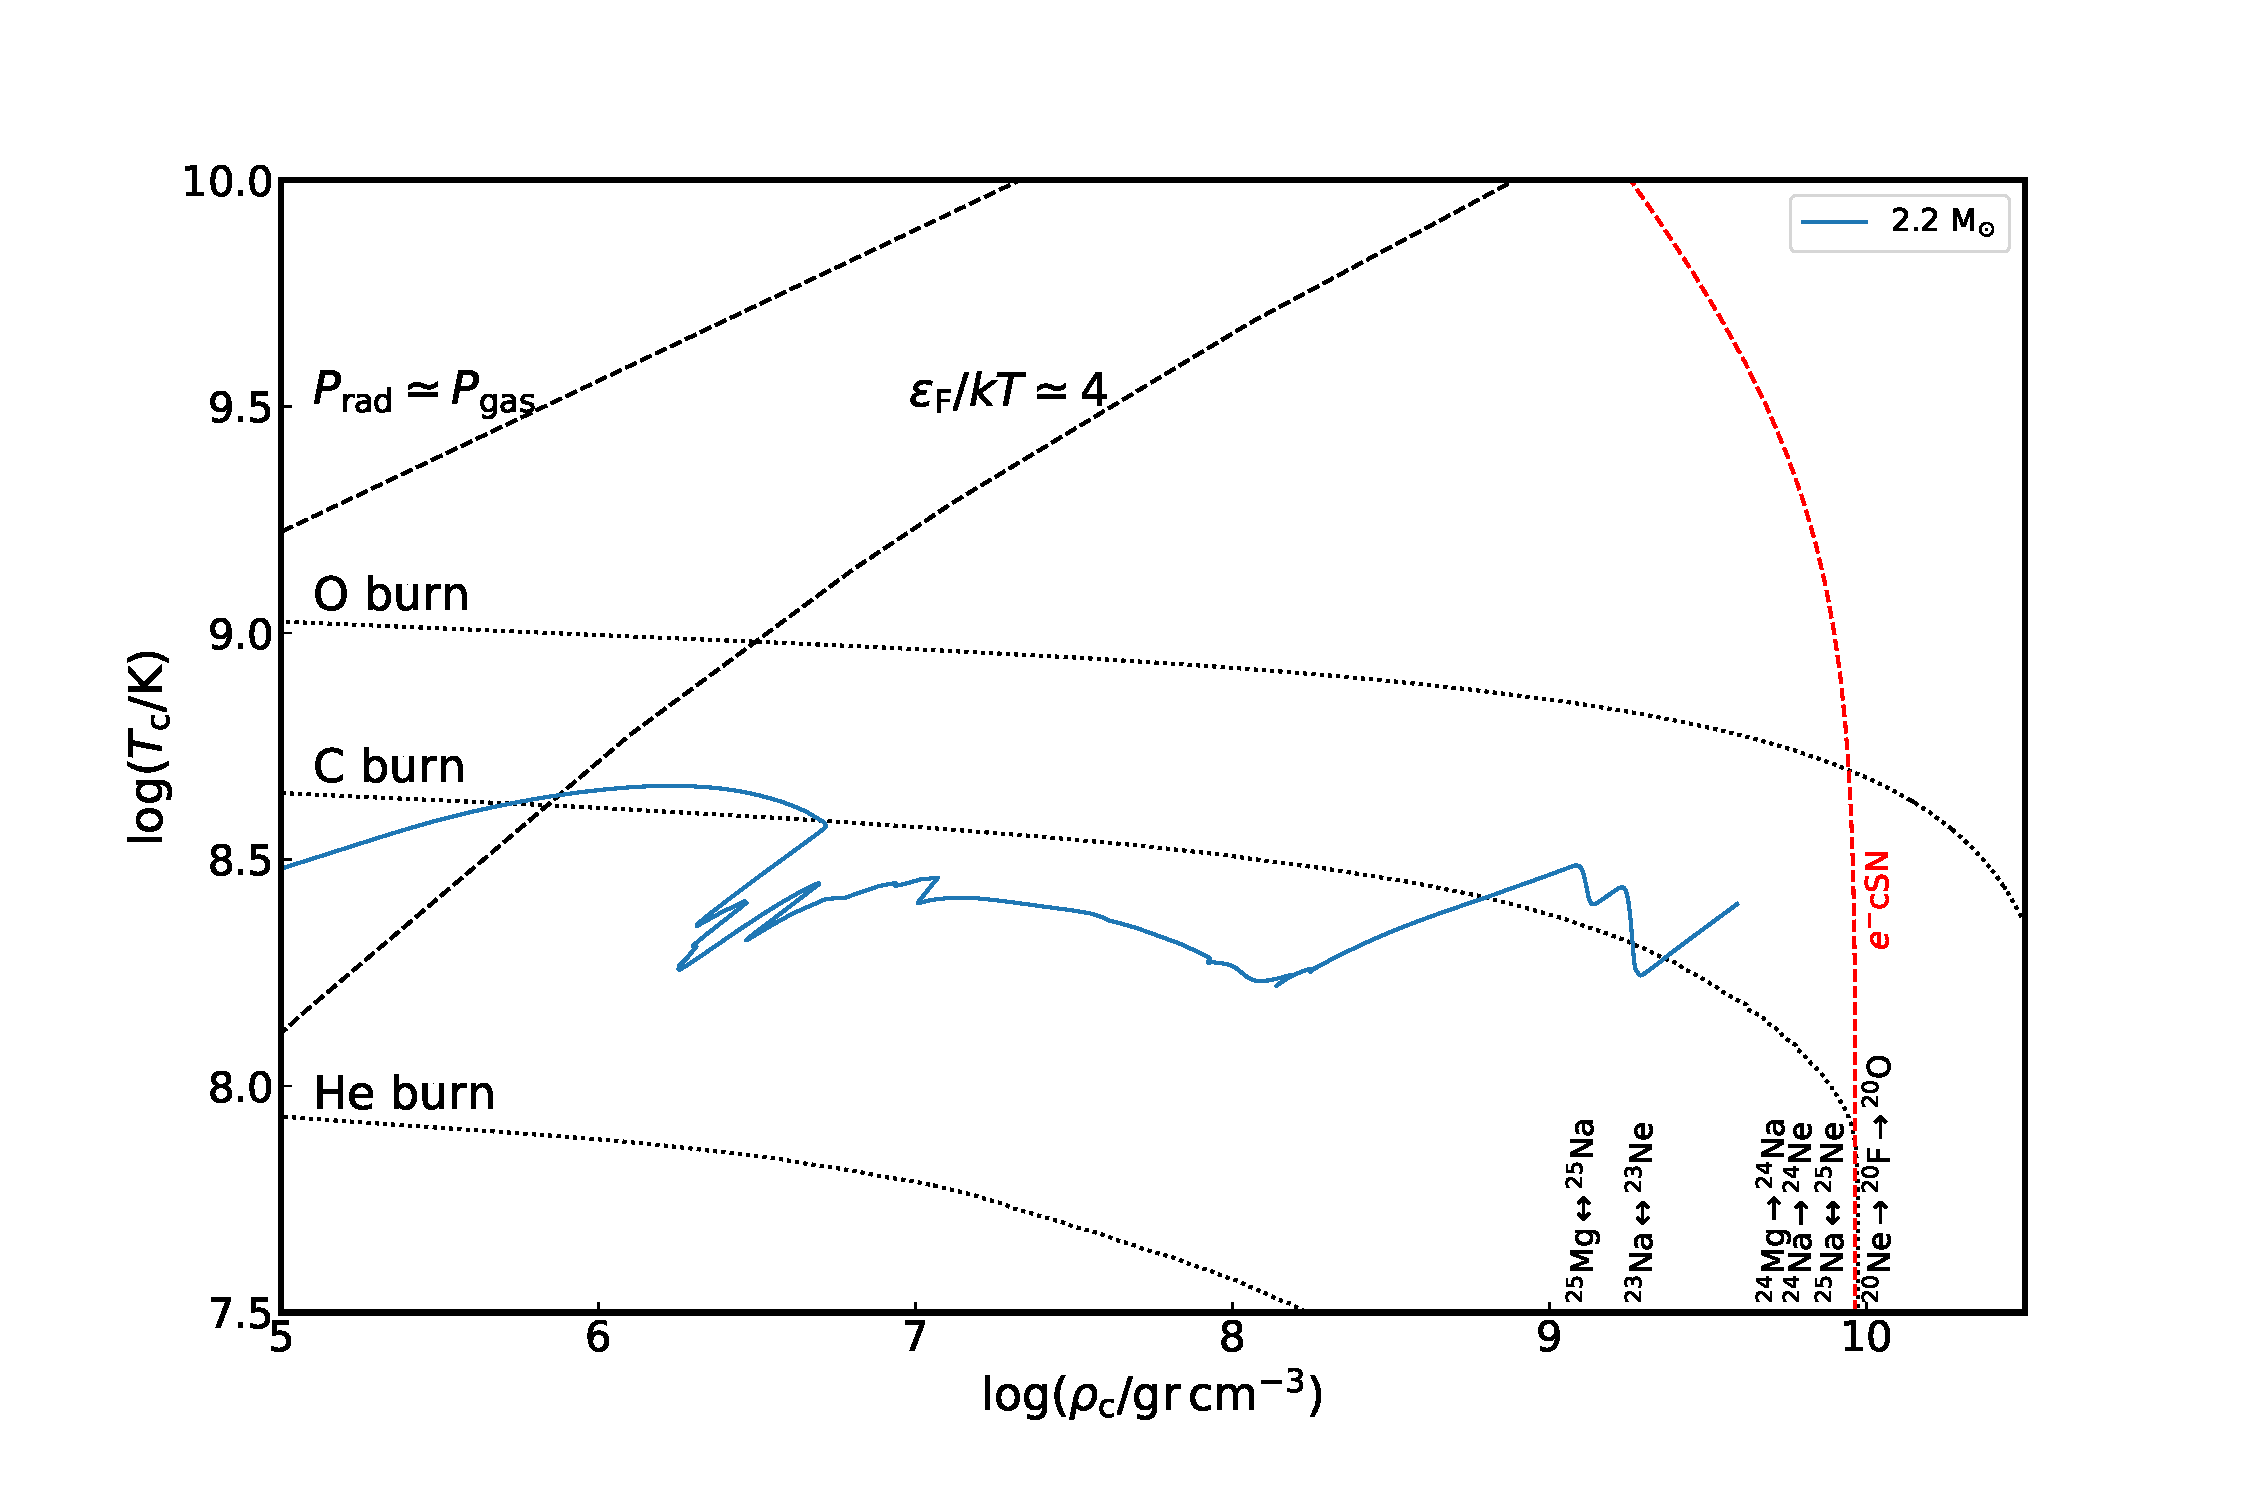
\includegraphics[width=1.0\textwidth]{Rhoc_vs_Tc.pdf}
\caption{Evolution of the core density and temperature }
\label{fig:rhocvst}
\end{center}
\end{figure*}


\section{Numerical models}\label{sec:3}
We use the \textit{Modules for Experiments in Stellar Astrophysics}  \citep[\textsc{mesa};][]{Paxton:2010ji} 
to construct a detailed numerical model for the evolution of two Helium cores
with masses of 1.8 and 2.3\,M$_{\odot}$.
These models as representative of the two possible scenarios described above: 
the former star develops a hybrid CO/ONe structure while the 
latter evolves onto an ONeMg core. 
A complete grid of single He stars with masses between 1.5 and 3.5\,M$_{\odot}$ 
is presented in a companion paper by Chanlaridis et al. 2019. 

\textsc{mesa} is an implicit 

\subsection{Input Physics}

\subsection{}


\textsc{mesa} solves the stellar structure and evolution 
equations using an implicit Langrangian scheme. 

\section{Energetics}

\section{Rates}
To first order, the \emph{maximum} number of SN\,Ia per unit mass is:

\begin{equation}
n_{\rm SN\,Ia} \simeq n_{\rm sAGB}\times f_{\rm bin} \times f_{\rm CE},
\end{equation}
where 


Hubble-time integrated number of SN\,Ia is $\sim 2\pm 1$\,per\,1000\,M$_{\odot}$. 
Number of stars able to develo He cores with masses between 
1.8 and 2.5\,M$_{\odot}$ if they enter a CE before the sDU episode is 
$n_{\rm sAGB}\simeq 9.6$\,per\,1000\,M$_{\odot}$ 
assuming a \cite{habrier:2004vw} initial mass function. 


Alternative approach: number of systems that give 
\section{Discussion}

Summarise. Say how they they would interact with a binary etc. Explosion physics, 
summarise results of Nomoto group and explosion simmulations are higher densities. 






\software{MESA\footnote{http://mesastar.org} \citep{Paxton:2010ji,Paxton:2013pj,Paxton:2015jva,Paxton:2017eie},
          Astropy\footnote{http://www.astropy.org} \citep{Robitaille:2013mpa,Price-Whelan:2018hus}}

\bibliography{refs}
\bibliographystyle{yahapj}


\end{document}

